% =====================================================================
% Robust but scale-dependent digital phenotypes of mental disorders
% Nature Human Behaviour 鈥?Article (main text)
% Compile: pdflatex digital_phenotyping_NHB.tex (twice). Figures in ./figures/
% Numbers frozen in paper_claims_allowed_wording.md and checked by check_numbers.py.
% Style: unheaded Introduction; descriptive Results subheadings; Results-first
% sentences; Discussion without subheadings (NHB house style).
% NHB Article limits: main text <=5,000 words; abstract <=150 words; <=8 display items;
% unlimited references; Extended Data <=10.
% =====================================================================
\documentclass[11pt]{article}
\usepackage[margin=1in]{geometry}
\usepackage[T1]{fontenc}
\usepackage[utf8]{inputenc}
\usepackage{mathptmx}
\usepackage{graphicx}
\usepackage{booktabs}
\usepackage{amsmath,amssymb}
\usepackage{color}
\usepackage{setspace}
\singlespacing
\usepackage{caption}
\DeclareCaptionLabelSeparator{pipe}{\ \textbar\ }
\captionsetup[figure]{name=Fig., labelsep=pipe, font=small, labelfont=bf,
  singlelinecheck=false, justification=raggedright, skip=3pt}
\captionsetup[table]{font=small, labelfont=bf, singlelinecheck=false,
  justification=raggedright, skip=3pt}
\setcounter{topnumber}{2}\setcounter{bottomnumber}{2}\setcounter{totalnumber}{4}
\renewcommand{\topfraction}{0.9}\renewcommand{\bottomfraction}{0.9}
\renewcommand{\textfraction}{0.07}\renewcommand{\floatpagefraction}{0.75}
\usepackage{lineno}
\usepackage[colorlinks=true,urlcolor=blue,citecolor=blue]{hyperref}
\newcommand{\doi}[1]{\href{https://doi.org/#1}{doi:#1}}
\newcommand{\supfig}[1]{Supplementary Fig.~#1}
\newcommand{\suptab}[1]{Supplementary Table~#1}
\newcommand{\edfig}[1]{Extended Data Fig.~#1}

\begin{document}
\linenumbers

\begin{center}
{\LARGE\bfseries Robust but scale-dependent digital phenotypes of mental \\[4pt]
disorders in 128{,}000 Reddit users}

\vspace{0.9em}
{\large Author One$^{1}$, Author Two$^{2}$, Another Author$^{1}$,
Corresponding Author$^{1,\ast}$}

\vspace{0.4em}
{\small $^1$Affiliation One; $^2$Affiliation Two.\\
$\ast$Correspondence: corresponding@institution.edu}

\vspace{0.7em}
{\small \emph{Draft for Nature Human Behaviour (Article). Extended Data figures and
Supplementary Information are provided in \texttt{extended\_data\_NHB.tex} and
\texttt{supplementary\_information\_NHB.tex}.}}
\end{center}

\begin{abstract}
\noindent Digital phenotyping promises passive, scalable measurement of mental health, but its
validity may not transfer across levels of inference. We analysed 128{,}003 Reddit users who
self-reported a diagnosis across ten disorders and 595{,}571 propensity-matched comparison users
(2006--2023), evaluating digital phenotypes across five scales. Multidimensional features
distinguished users who reported a diagnosis from comparison users (area under the receiver
operating characteristic curve, AUROC, 0.84--0.92), with little change after excluding
diagnosis-triggering posts (mean $\Delta$AUROC 0.006). Yet cross-diagnostic patterns were
predominantly shared and dimensional rather than categorical (adjusted Rand index 0.088), and
individual change-points around the self-reported diagnosis were too sparse to support reliable
early warning. Discriminability was not significantly aligned with independently sourced
comorbidity (Mantel $r=-0.25$, $P=0.30$). At population scale, correcting a composition-induced
temporal bias reversed the apparent trend in the digital p-factor; after accounting for temporal
trends, behavioural volatility remained associated with national suicide mortality (detrended
$r=0.47$), whereas language-based severity did not show a comparably robust association. These
findings show that group-level discrimination does not establish diagnostic specificity,
individual early-warning capacity or population-monitoring validity. Digital phenotypes must
therefore be evaluated separately at each scale of inference.
\end{abstract}

% ---------------------------------------------------------------- Introduction (no heading)
\section*{Introduction}
Digital traces of everyday behaviour are increasingly used to measure psychological states, and digital phenotyping---the inference of mental-health states from passively collected digital behaviour
\cite{insel2017digital,insel2018global,onnela2016harnessing,torous2017dimensions} and is
widely proposed as a scalable complement to clinical assessment. Smartphones and social
platforms record behaviour continuously and unobtrusively, and language and activity are
repeatedly associated with depression and other conditions
\cite{dechoudhury2013predicting,coppersmith2014quantifying,coppersmith2015adhd,
eichstaedt2018facebook,guntuku2017detecting}. Against this promise, the field has been
criticized for over-claiming: effects are often modest, samples small or confined to a single
disorder, and the actionable value of a correlational signal is unclear
\cite{braund2024hype,orben2019association,panayiotou2023time,adam2025smartphones}. The missing
element is not another single-disorder classifier but a systematic answer to a prior question:
at which scale of inference are digital phenotypes valid, and in what form
\cite{giampetruzzi2026promise,lord2023autism}. The question is not rhetorical. A model that
separates groups at AUROC 0.90 may still be useless for an individual, because a group-level
contrast does not define a decision boundary for one person; conversely, a feature that is
uninformative for individual classification may be a sensitive population indicator. The same
data can therefore support, or fail to support, quite different claims depending on the
inference target, and those targets are rarely separated within a single study.

Behavioural and linguistic traces carry psychological signal in ways that are well
characterized but fragmented. Linguistic style is a stable individual difference
\cite{pennebaker1999linguistic,pennebaker2003psychological,schwartz2013personality,
kern2014online}; depressed individuals use more first-person singular and negative-emotion
words \cite{rude2004language,stirman2001word}; absolutist language marks anxiety, depression
and suicidal ideation \cite{almosaiwi2018absolute}; and, at scale, Facebook language predicts
depression recorded in medical notes \cite{eichstaedt2018facebook}. Language also carries
community-level health signal \cite{eichstaedt2015heart}, although such ecological claims
demand multiplicity and validation controls \cite{brown2018replicationstatements}. A second,
partly independent channel is behavioural: posting rhythm, social withdrawal and activity
variability accompany psychiatric states
\cite{dechoudhury2016discovering,coppersmith2014quantifying}. Because diagnoses are
heterogeneous, markers can also depend on demographic context
\cite{rai2024race,defreitas2024black,wang2024llm,hur2024sentiment}, and cognitive-linguistic
features track specific psychopathology dimensions \cite{fradkin2025language}; large language
models are increasingly proposed as psychometric instruments \cite{capraro2025llmwellbeing},
so linguistic markers warrant caution about construct validity.

Three questions organize the accumulating but disconnected evidence. First, is the digital
phenotype categorical or dimensional: do disorders map onto separable digital signatures, or
onto largely shared dimensions? Clinical psychiatry increasingly describes a general
psychopathology factor and hierarchical-spectrum organization
\cite{caspi2014p,kotov2017hitop,rodriguezseijas2023diversity,pnas2023pfactor}, but whether
passively measured digital phenotypes reproduce that structure, or are dominated by one shared
dimension, has not been tested at scale. Second, is the goal individual detection or
population monitoring: are the features that flag an individual the same features that track a
population? Large quasi-experimental and natural-experiment studies show that platform exposure
and societal shocks can shift mental-health outcomes
\cite{braghieri2022social,allcott2020welfare,shi2026protests,roozenbeek2026protests,
skeggs2025interventions,fassi2025adolescents,pearson2025smartphones}, which makes the scale of
validity a practical question: if a phenotype is valid only in part of the inference space,
both monitoring and intervention may target the wrong layer. Third, where are the temporal
boundaries: can individual transitions be anticipated, or is the per-individual signal too
sparse \cite{giampetruzzi2026promise,dechoudhury2016discovering}?

Here we assemble the largest matched case--control social-media cohort of its kind:
128{,}003 users with self-reported diagnoses across ten disorders and 595{,}571
propensity-matched comparison users from Reddit (2006--2023), described by 101 candidate
behavioural, linguistic, temporal and social features. Analyses are reported at one of three
nested cohort layers of the same matched sample: the matched layer (128{,}003/595{,}571)
provides the cohort and matching statistics, the feature layer (127{,}168/594{,}817) the
individual-phenotype analyses, and the trajectory layer (123{,}986/565{,}598) the longitudinal
and population analyses; each figure states the layer it uses. We test five scales of
inference---individual detection, disorder-versus-disorder separation, latent structure,
individual early warning, and population monitoring---and, separately, a methodological audit
of a composition bias that can fabricate population trends (Fig.~\ref{fig:design}c,d). We treat the resulting map not as a single classifier but as a statement
about where each class of claim is supportable, and where it is not; our central finding is that discriminability at one scale does not transfer to validity at another, so each scale must be evaluated on its own terms. All data are public Reddit
posts analysed in anonymised form; no contact, intervention or re-identification was performed,
and self-reported labels are not clinical diagnoses (Methods, ``Data source and cohort construction'').

\section*{Results}

\subsection*{A reproducible, multidimensional digital phenotype atlas}
The matched layer contained 128{,}003 users with self-reported diagnoses and 595{,}571 matched comparison users
(attention-deficit/hyperactivity disorder (ADHD) 37{,}645; depression 30{,}645; anxiety 14{,}426; autism 10{,}225; bipolar disorder 10{,}007; post-traumatic stress disorder (PTSD)
8{,}282; borderline personality disorder 6{,}083; obsessive--compulsive disorder (OCD) 5{,}736; schizophrenia 2{,}461; eating disorders
1{,}688; 805 unlabelled) (Fig.~\ref{fig:design}a,b; \suptab{1}). Matching balanced activity
history closely (maximum standardised mean difference 0.054 before and 0.0097 after
inverse-probability weighting; effective sample size 586{,}010); 39{,}059 users (30.5\%)
carried two or more diagnoses, most often anxiety--depression (15{,}140)
(\supfig{3}). Across 930 non-artefact feature--disorder tests, 765 (82.3\%) were significant
after Benjamini--Hochberg control, but effect magnitude was modest: mean $|$Hedges'
$g|=0.21$ (median 0.12; interquartile range 0.04--0.27; 95th percentile 0.76)
(Fig.~\ref{fig:atlas}a--c). No single marker dominated the atlas, and the
distribution of $|g|$ was right-skewed with most effects in the small-to-moderate range. These effects were stable across subsampling, confounder adjustment
and temporal thirds (Fig.~\ref{fig:atlas}c; \supfig{1}; \suptab{1}), indicating that the
atlas reflects a reproducible property of the cohort rather than a fragile artefact of one
analysis.

Users with self-reported diagnoses were distinguished from matched comparison users with an area under the
receiver operating characteristic curve (AUROC) of 0.84--0.92 across the ten disorders
(Fig.~\ref{fig:atlas}d). Because users write \emph{about} their diagnoses, part of this
separability could reflect diagnosis-related language rather than phenotype; when
diagnosis-triggering posts were excluded and features recomputed, discrimination was largely
preserved (mean $|\Delta$AUROC$|=0.006$; only anxiety, $-0.017$, and depression, $-0.015$,
attenuated modestly), indicating that the signal is not driven solely by diagnosis language
(Fig.~\ref{fig:atlas}e; \edfig{1}). Removing whole feature families degraded discrimination
unevenly---affective features retained AUROC 0.825, temporal features fell to 0.597, and all
families together reached 0.886 (Fig.~\ref{fig:atlas}f)---so the phenotype is
multidimensional rather than a single sentiment axis, consistent with evidence that language
markers are context-dependent \cite{rai2024race}. Per-class confusion and multiclass
coefficients are detailed in \edfig{3}, feature-level robustness in \edfig{2}, and the full
sensitivity suite and further feature-level detail in \supfig{1} and \supfig{2}.

\subsection*{A reproducible transition but no reliable individual early warning}
We divided each user's history into 90-day windows advanced in 30-day steps (adjacent windows
therefore overlap by 60 days) and spanning $t_0\pm720$ days, indexing each window by its centre
relative to the self-reported diagnosis date $t_0$. Across these windows the case-minus-comparison
gap in the \emph{digital p-factor}---a researcher-defined severity composite built from the
cross-disorder first-factor loadings (Methods, ``Trajectory construction and the p-factor'')---was
approximately $-0.07$ at day $-675$, converged toward zero before $t_0$, peaked
transiently at $+0.12$ around $+15$ days, and returned to near zero by $+225$--$285$ days before
drifting slightly negative (Fig.~\ref{fig:temporal}a). The morphology is coherent---a modest,
time-localized elevation that decays---rather than a step change sustained after the report date.
The pre-trend was not parallel (17 of 22 pre-diagnosis windows were significant after
false-discovery-rate control), so the transition is described rather than given a causal
interpretation (\edfig{6}); a difference-in-differences estimate of the p-factor is
correspondingly small ($+0.020$; volatility $+0.037$; withdrawal $-0.042$;
Fig.~\ref{fig:temporal}d), and a 100-draw placebo in which the pseudo-diagnosis date was shifted
produced a null that the observed estimate does not separate from, so we treat the causal reading
as inconclusive.

Per-user change-point detection found 1{,}309 change-points in total, spread across 887 users;
of these users, only 67 had any change-point before $t_0$ (overall median lead 161 days), so
reliable per-individual early warning is \emph{not supported} by these data
(Fig.~\ref{fig:temporal}c; \edfig{6}). Thus the 1,309 is a total change-point count from the
whole cohort, the 887 is the number of users contributing them, the 67 is the number of users
with a change-point before their report date, and Fig.~\ref{fig:temporal}c displays the five
disorder groups contributing more than five such users, which together account for 54 of the 67
affected users. The negative result is a property of the signal's sparsity rather than of the
estimator: the boundary is robust to the imputation assumption because individual-level
analyses use only reliable windows (Methods, ``Trajectory construction and the p-factor'';
\edfig{9}), and it is stable across the change-point penalty (\edfig{6}d). The transition
itself, by contrast, reproduced across calendar eras---the surge gap was 0.105/0.107/0.109
across three eras, and a classifier trained in one era and tested in another on the identical
atlas lost little performance (mean $|\Delta$AUROC$|=0.010$; deltas $-0.013$, $-0.012$,
$+0.004$) (Fig.~\ref{fig:temporal}e,f; \edfig{1}). Gaussian-mixture subtyping (exploratory;
$k=2$ chosen by silhouette, not Bayesian information criterion) separated a large
``acute-on-chronic'' trajectory (93.8\%), already elevated before $t_0$ and stepping up at it,
from a small ``fluctuating'' trajectory (6.2\%) with high within-window variability
(Fig.~\ref{fig:temporal}b; \edfig{5}).

\subsection*{Predominantly shared, dimensional cross-diagnostic structure}
Across all 45 disorder pairs, case-versus-case discrimination was moderate: the mean AUROC was
0.741 on the 108-feature cross-diagnostic set (the 93-feature atlas extended with log-transformed variants used for pairwise classification), ranging from 0.63 for anxiety--OCD to 0.83 for autism--eating
disorders (Fig.~\ref{fig:structure}a; \edfig{1}). A two-dimensional embedding of 18{,}000 users showed
disorder centroids overlapping with no discrete clusters (permutation separation $P=0.31$),
and the HiTOP \cite{kotov2017hitop}, DSM-5 \cite{apa2013dsm5} and comorbidity structural-fit correlations were all non-significant
(Fig.~\ref{fig:structure}b; Methods). The clustering that best fits the data separated a single
large group, with only autism apart (silhouette 0.653; 9 of 10 disorders in one cluster),
reinforcing the absence of clean categorical boundaries.

Factor analysis of the 93$\times$10 effect-size matrix yielded a single dominant dimension
(Factor 1, 94\% of variance; the three-factor solution is an analyst/HiTOP choice, with
data-driven parallel analysis suggesting two factors and a three-factor cumulative variance of
97.5\%) (Fig.~\ref{fig:structure}c; \edfig{4}). This first factor resembles a general
psychopathology-like dimension at the digital level, but it is a cross-disorder structure of
effects, not an individual clinical p-factor; its loadings mix affective, temporal and activity
features in a way that does not map onto a single clinical axis. Hierarchical clustering agreed
poorly with HiTOP (adjusted Rand index 0.088) and 69\% of network edges were shared by five or
more disorders (Fig.~\ref{fig:structure}e,f; \edfig{7}; \supfig{3}), so the structure is best
described as \emph{shared and dimensional}, echoing transdiagnostic network accounts of
psychiatric illness \cite{hitopnetwork2023}.

Higher case-versus-case separability was only directionally related to independently sourced
clinical comorbidity (21 DOI-referenced pairs, with sources listed in \suptab{4}; Mantel
$r=-0.247$, $P=0.30$; Spearman $r=-0.095$, $P=0.68$); the
association was directionally consistent but not statistically significant
(Fig.~\ref{fig:structure}d; \supfig{3}). A same-cohort empirical comorbidity matrix
correlated positively with digital distances ($r=+0.40$, $P=0.008$), but this reflects
internal consistency only and not external convergence (Methods, ``Discrimination, leakage and structure''; \supfig{3}). The phrasing
throughout is therefore ``consistent with a dimensional representation'', not a demonstration
of it.

\subsection*{Population behavioural signals track societal perturbations}
Reliable windows were aggregated onto a monthly grid (17.25 million windows; Methods, ``Population aggregation and time-series models''); the resulting case-minus-comparison series for four signals is shown in Fig.~\ref{fig:population}a. In a
window-level regression that controlled for time-from-diagnosis and calendar month, the onset
of COVID-19 coincided with a behavioural-volatility shift of $+0.046$ ($P\approx10^{-18}$) and
a small p-factor shift of $+0.010$, with posting $-0.113$ and social withdrawal $-0.012$
(Fig.~\ref{fig:population}b,d; \edfig{8}). The shift was not uniform across disorders: the
same sign appeared for most, but its size varied, and the trend change after the breakpoint was
more consistent than the level shift (Fig.~\ref{fig:population}e), suggesting a slow
reorganisation of posting behaviour rather than a single shock; the per-disorder volatility
series is shown in Fig.~\ref{fig:population}f. Applying the same design to five societal events, only the 6
January 2021 US Capitol attack showed a robust severity (p-factor) gap ($+0.011$,
$P=3.6\times10^{-7}$); the 2020 Black Lives Matter period was weaker ($-0.005$, $P=0.046$) and
the 2016 election, the 2018 celebrity-suicide period and the immediate COVID window were not
significant (Fig.~\ref{fig:population}c). Not every salient event yields a population
behavioural signal, and the pattern is coincident rather than causal.

\subsection*{Composition-induced temporal bias can reverse population conclusions}
Users' calendar-time position relative to their self-reported diagnosis drifted over
2006--2023, so naive calendar aggregation mixed event-time windows differently in early and
late years. This composition-induced temporal bias manufactured a spurious trend in the naive
p-factor series (Mann--Kendall $\tau=+0.31$); after balancing event-time composition by band
adjustment and a window-level regression, the trend reversed to $\tau=-0.31$ ($P=0.16$; no
trend) (\edfig{10}). That a population trend can flip sign under
a purely compositional correction is the central methodological point: the naive series is not
a weaker version of the corrected one, but a different estimand. The practical consequence is
that population monitoring which aggregates event-aligned behavioural data over calendar time
can report a trend that is an artefact of who enters the sample when; reporting the
composition-adjusted series is therefore a precondition for any population-trend claim. In a
three-scenario simulation, pure composition drift with no true trend produced a spurious
significant naive trend ($\tau=+0.77$), whereas the adjusted estimators returned a null and
scenarios with a true trend were recovered (\edfig{10}). The resulting principle---balance
event-time composition before calendar-time aggregation---is a reusable audit for population
digital mental health, and is not specific to this cohort or platform.

\subsection*{Behavioural volatility, not language, carries the external signal}
Band-adjusted annual behavioural volatility covaried with national suicide mortality (CDC
underlying-cause-of-death data, ICD-10 X60--X84, age-adjusted per 100{,}000; raw
$r=0.906$ with bootstrap 95\% confidence interval 0.77--0.97; first-difference $r=0.511$;
detrended $r=0.473$; permutation $P<0.001$; leave-one-year-out range of $r$ 0.03)
(Fig.~\ref{fig:external}a--e; \edfig{8}). The association survived first-differencing and
detrending, the two transformations that most credibly remove shared secular trends, and it was
stable when single years were removed, and its correlation was consistent across adjacent
lags, which argues against a purely mechanical common trend.
The language-based severity composite did not survive detrending, and posting intensity was
only directionally related (detrended $r=-0.39$) (Fig.~\ref{fig:external}f). This association
is ecological and population-level; it is explicitly \emph{not} individual-level suicide
prediction, and Reddit users are not the general population (Methods, ``External validation''; \suptab{2}). Taken
together, the features that flag individuals do not monitor populations: behavioural
volatility, rather than language-based severity, carries the population-level external signal.

\section*{Discussion}
Digital phenotyping is often discussed as if validity were a single property, but the present
results show that it is a property of a scale, a target and an estimand. Across five scales,
we found a clear structure to what is and is not supportable. Individual detection is strong
(AUROC 0.84--0.92) and not driven solely by diagnosis language; disorder-versus-disorder
separation is moderate; discrete categorical structure is unsupported, the structure being
shared and dimensional; individual early warning is not supported by these data; and population
monitoring is carried by behavioural volatility rather than language. The practical consequence
is that a digital phenotype should be described with the scale at which it operates attached to
it, in the same way that a biomarker is described with its reference population and assay. Table~\ref{tab:capability} summarises this capability map, and each verdict rests on the evidence at that scale rather than on performance elsewhere.

Detection is not prediction. That users with self-reported diagnoses are distinguishable from matched comparisons
does not imply that the same signal can anticipate an individual's transition. The
event-time transition was real and reproducible across eras, but it was not parallel-trends
compliant, and pre-diagnosis change-points were too sparse to support reliable early warning.
We present this boundary as a result: the honest contribution is to show where individual
prediction fails, not to promise early detection \cite{giampetruzzi2026promise}. This is
consistent with the observation that group-level separability and individual-level prediction
are governed by different quantities, so that high AUROC and poor single-person forecasting can
coexist.

The digital structure was shared and dimensional rather than a set of separable diagnoses:
disorder centroids overlapped, the first factor dominated, clustering agreed poorly with HiTOP,
and most network edges were shared across disorders. This is \emph{consistent with} dimensional
models of psychopathology \cite{caspi2014p,kotov2017hitop} rather than proof of them, and the
external comorbidity convergence was non-significant; the dimensional vocabulary should be
used with that caution. The finding also carries a design implication: if the digital phenotype
is dominated by a single shared axis, then feature sets chosen to separate one disorder from
controls will largely re-express that axis, and transdiagnostic rather than disorder-specific
features are the appropriate target for cross-diagnostic work.

The features that detect individuals and those that monitor populations differ. Behavioural
volatility covaried with national suicide mortality after detrending, whereas language-based
severity did not; this cautions against transferring individual-level feature importance to
population monitoring, and vice versa \cite{shi2026protests,roozenbeek2026protests}. Calendar
aggregation of event-aligned data can additionally fabricate population trends when composition
drifts; the simulation-validated audit we provide---band adjustment and window-level
regression---reverses a naive trend and recovers the truth under known scenarios, and is a
standard check we recommend for population digital mental-health monitoring
\cite{eichstaedt2015heart,brown2018replicationstatements}. Because cohort composition drifts
whenever the sampling frame and the outcome are both time-varying, the risk is not specific to
Reddit or to mental health.

Several boundaries constrain these claims without overturning the within-design results.
Self-reported diagnoses are a silver-standard proxy, not clinical records; the report date is
not the date the illness began; behaviour is a proxy for the diagnosis, not the diagnosis
itself; Reddit
users are not representative of the general population; the external series are short and
ecological; the external comorbidity convergence was non-significant; and misclassification of
self-report status is non-zero. We quantify sensitivity wherever assumptions are load-bearing
(Methods, ``Statistics, software and reproducibility''; \edfig{9}; \suptab{3}). The appropriate uses of this phenotype are
population-level monitoring and timing-aware support, not automated diagnosis or individual
risk scoring; deployment should be accompanied by data governance, explicit consent for any
non-public data, and a clear prohibition on re-identification, and the composition-bias audit
should be part of routine reporting \cite{braund2024hype,pearson2025smartphones}.

\section*{Methods}

\subsection*{Data source and cohort construction}
Reddit comments and submissions (2006--2023) were assembled from a public Pushshift snapshot of
monthly ZST-compressed dumps. In a first phase, case identification scanned every post (submission title and
self-text; comment body) in four stages. A candidate had to match the first-person inclusion
grammar
\begin{equation}
\texttt{I (?:was|have been|am|got) (?:officially|clinically|formally|professionally)? diagnosed with [\ldots]}
\label{eq:inc}
\end{equation}
(case-insensitive). A hit was then rejected if it contained an exclusion cue (self-diagnosed; a
third-party possessor such as \emph{my mom/dad/friend/partner}; not or never diagnosed;
mislabeled or misdiagnosed), leaving 77+ disorder keywords spanning DSM-5/ICD-11 terminology
and Reddit vernacular across the ten disorders. Retrospective time expressions
(\texttt{n years/months/weeks ago}, \texttt{in 19xx|20xx}, \texttt{when I was},
\texttt{since \ldots}) were flagged as \texttt{is\_retrospective} but not rejected. Finally, a
\texttt{spaCy} dependency gate required a token with \texttt{lemma = diagnose} and
\texttt{pos = VERB} whose subject or object (nsubj/nsubjpass/dobj) was first-person
(\emph{i/me/my}) and which was not negated; only then was a post treated as a valid
self-reported diagnosis, with $t_0$ the earliest such post and all endorsed disorders recorded.
In a second phase, the complete posting history (posts and comments) of every identified
user and of non-hit comparison candidates (sampled at rate 0.001 with $\ge$5 history posts),
regex-replacing URLs and emails with placeholder tokens. Bot and quality filtering applied the
thresholds
\begin{equation}
\texttt{posts\_per\_day}\le 60,\quad \texttt{avg\_word\_len}\ge 2.5,\quad
\texttt{vocab\_density}\ge 0.3,\quad \texttt{tenure}\ge 30~\mathrm{d},\quad \texttt{total\_posts}\ge 5,
\label{eq:bot}
\end{equation}
also removing newly created, high-frequency accounts; this retained 4{,}771{,}571 of
4{,}950{,}144 posts ($\approx$3.6\% removed as suspected bots). A shadow-$t_0$ was drawn for
each comparison user from the empirical distribution of diagnosed-user $t_0$ values, requiring $\ge$30~d
of history either side (3{,}730{,}213 users). Identifiers are salted SHA-256 hashes (collision
$\approx$0.1--0.2\%) and personally identifying information was redacted. A Silver layer then
re-sharded all posts by user (\texttt{user\_id\_hash[:5] mod 500}) into a 30-column schema with
clinical flags (\texttt{is\_diagnosis\_post}, \texttt{is\_retrospective}, \texttt{flag\_suicide},
\texttt{flag\_self\_harm}) to give every downstream module a single stable interface. The
resulting label is a self-reported diagnosis (a behavioural proxy), not a clinical record.

\subsection*{Propensity-score matching and weighting}
Let $T_i\in\{0,1\}$ indicate a user with a self-reported diagnosis and $\mathbf{x}_i$ the 11 activity-history
covariates (log posts per day, log tenure, readability grade, subreddit entropy, submission
ratio, circadian hour sine and cosine, circadian regularity, vocabulary density, log total
posts, active-day ratio). A propensity score was estimated by logistic regression
\cite{rosenbaum1983central,stuart2010matching},
\begin{equation}
e(\mathbf{x}_i)=\Pr(T_i=1\mid \mathbf{x}_i)=\bigl[1+\exp(-\beta_0-\boldsymbol{\beta}^{\!\top}\mathbf{x}_i)\bigr]^{-1},
\label{eq:ps}
\end{equation}
and matching was performed within exact \texttt{tenure\_quartile} strata on the logit propensity
$\ell_i=\log\{e(\mathbf{x}_i)/[1-e(\mathbf{x}_i)]\}$, using nearest-neighbour matching without
replacement at a 1:5 ratio and a caliper of 0.2 standard deviations of $\ell$ within each
stratum (seed 2025). Balance was summarised by the standardised mean difference
\begin{equation}
\mathrm{SMD}=\frac{\bar{x}_{T}-\bar{x}_{C}}{\sqrt{(s_{T}^{2}+s_{C}^{2})/2}},
\label{eq:smd}
\end{equation}
maximised over covariates, where $\bar x_{T},\bar x_{C}$ and $s_{T},s_{C}$ are the diagnosed-user
and comparison means and standard deviations (weighted forms under inverse-probability weighting). Residual imbalance was addressed by stabilised
inverse-probability-of-treatment weighting,
\begin{equation}
w_i=\frac{T_i}{\hat e_i}+\frac{1-T_i}{1-\hat e_i},
\label{eq:iptw}
\end{equation}
with the propensity score trimmed at its 5th/95th percentiles and weights capped at the 99th
percentile, and by entropy balancing as a sensitivity analysis. The effective sample size was
$\mathrm{ESS}=(\sum_i w_i)^2/\sum_i w_i^2$. Matching and weighting reduced the maximum SMD from
0.054 to 0.0097 and gave an ESS of 586{,}010. Rosenbaum sensitivity was assessed over
$\gamma\in[1,3]$. Three nested layers are reported: L1 (matched, 128{,}003/595{,}571), L2
(feature-quality filtered, 127{,}168/594{,}817) and L3 (trajectory-eligible,
123{,}986/565{,}598) (\suptab{1}).

\subsection*{Feature construction and normalisation}
Per-post linguistic features were computed by regular expressions (URL/email, sentence and
pronoun structure, tense, negation and hedging markers, swear and emotion-word counts) and by
external dictionaries under a strict source policy (regular expressions, then LIWC2015 \cite{pennebaker2015liwc}, then the NRC emotion lexicon \cite{mohammad2013nrc}; 37 LIWC
categories; NRC emotion lexicon v0.92, 6{,}453 words); sentiment and emotion-lexicon features
used VADER \cite{hutto2014vader}, and movement-average type--token ratio was computed over
50-word windows. Posts were then aggregated to user-level rates (e.g.\ anxious-word rate as a
safe ratio of counts to total words) across 14 dimensions, together with reliability flags
(valid-post count; linguistic and temporal reliability; dictionary coverage). Three features
with zero training interquartile range were dropped and five features circular with case
identification (subreddit entropy and Herfindahl, and primary- and mental-health-subreddit
ratios) were excluded, leaving $p=93$ features and $10$ disorders. Each feature was winsorised
to the [0.5, 99.5] percentiles and robust-scaled \cite{pedregosa2011scikit},
\begin{equation}
\tilde{x}=\frac{x-\operatorname{median}(x)}{\operatorname{IQR}(x)},
\label{eq:robust}
\end{equation}
with the median and interquartile range fitted on the training split only; circular clock-time
features were encoded as sine and cosine pairs prior to scaling.

\subsection*{Effect sizes, weighting and multiple testing}
For each feature--disorder pair the standardised mean difference was computed with a
small-sample correction (Hedges' $g$),
\begin{equation}
g=J\,d,\qquad d=\frac{\bar{x}_{1}-\bar{x}_{2}}{s_{p}},\qquad
s_{p}=\sqrt{\frac{(n_{1}-1)s_{1}^{2}+(n_{2}-1)s_{2}^{2}}{n_{1}+n_{2}-2}},\qquad
J=1-\frac{3}{4(n_{1}+n_{2})-9},
\label{eq:hedges}
\end{equation}
with two-sided $P$ values from Welch's $t$ test,
\begin{equation}
t=\frac{\bar{x}_{1}-\bar{x}_{2}}{\sqrt{s_{1}^{2}/n_{1}+s_{2}^{2}/n_{2}}},\qquad
\mathrm{df}=\frac{(s_{1}^{2}/n_{1}+s_{2}^{2}/n_{2})^{2}}{\frac{(s_{1}^{2}/n_{1})^{2}}{n_{1}-1}+\frac{(s_{2}^{2}/n_{2})^{2}}{n_{2}-1}}.
\label{eq:welch}
\end{equation}
where $\bar x_{1},\bar x_{2}$ and $s_{1},s_{2}$ are the two group means and standard deviations
with sizes $n_{1},n_{2}$ and $N=n_{1}+n_{2}$. Pairs with fewer than ten users were set to missing. An inverse-probability-weighted variant
replaced the means and variances with their weighted counterparts using the effective sample
size $\mathrm{ESS}$ and weights trimmed to the [1, 99] percentiles. Multiplicity across the
$m=930$ tests was controlled by the Benjamini--Hochberg procedure \cite{benjamini1995controlling}:
with ordered $P$ values $p_{(1)}\le\dots\le p_{(m)}$, reject $p_{(1)},\dots,p_{(k)}$ for the
largest $k$ with $p_{(k)}\le (k/m)\,\alpha$. For each feature we also computed magnitude
concentration (specificity), a direction-aware differential specificity equal to direction
diversity $\times$ magnitude concentration $\times$ a magnitude floor
$\min(1,|g|_{\max}/0.15)$, and a clinical-utility score combining effect magnitude, direction
consistency and significance under fixed weight schemes.

\subsection*{Discrimination, leakage and structure}
Single-disorder discrimination used $L_2$-penalised logistic regression \cite{tibshirani1996regression},
\begin{equation}
\min_{\beta_0,\boldsymbol{\beta}}\;
-\sum_{i}\Bigl[y_i\log \sigma(z_i)+(1-y_i)\log\{1-\sigma(z_i)\}\Bigr]
+\lambda\lVert\boldsymbol{\beta}\rVert_{2}^{2},\qquad z_i=\beta_0+\boldsymbol{\beta}^{\!\top}\mathbf{x}_i,
\label{eq:logreg}
\end{equation}
where $y_i$ is the diagnosis indicator, $\sigma(\cdot)$ the logistic function and $\lambda$ the $L_2$ penalty strength selected by cross-validated AUROC; controls were subsampled to
$\max(3n_{\text{case}},5000)$, and five subsample trials with stratified five-fold
cross-validation were averaged. Leakage was tested by excluding diagnosis-triggering posts,
recomputing features and refitting, and separately by feature-family ablation (refitting with
each dimension removed) and by dimension-only models. Cross-diagnostic structure used 45 pairwise
case-versus-case classifiers on a 108-feature set (the 93 analysis features plus log-transformed
variants), each balanced to the minority class; an embedding from
principal-component analysis (50 components) followed by UMAP
($n_\text{neighbors}=30$, $\texttt{min\_dist}=0.1$) \cite{mcinnes2018umap}; a graphical-lasso
network that estimates a sparse inverse covariance \cite{friedman2008sparse},
\begin{equation}
\hat{\Theta}=\arg\min_{\Theta\succ0}\;\operatorname{tr}(S\Theta)-\log\det\Theta
+\alpha\lVert\Theta\rVert_{1},
\label{eq:glasso}
\end{equation}
where $S$ is the empirical covariance, $\Theta$ its inverse, $\alpha$ the lasso penalty
(analyst-set at $0.8$, with an $\alpha$ sensitivity sweep) and $\lVert\cdot\rVert_1$ the
entrywise $\ell_1$ norm; average-linkage hierarchical
clustering on $1-\mathrm{AUROC}$; and factor analysis of the $93\times10$ effect matrix by
eigendecomposition of its correlation matrix with varimax rotation, retaining three factors (an
analyst/HiTOP choice; parallel analysis suggested two; the three-factor cumulative variance was
97.5\%). Agreement with HiTOP was measured by the adjusted Rand index. Separability was related
to an externally sourced, DOI-referenced comorbidity matrix by a Mantel test,
\begin{equation}
r_{\mathrm{M}}=\operatorname{corr}\bigl(\mathrm{vec}(U_A),\mathrm{vec}(U_B)\bigr),\qquad
P=\frac{1+\#\{|r_{\mathrm{M}}^{(b)}|\ge|r_{\mathrm{M}}|\}}{1+B},
\label{eq:mantel}
\end{equation}
where $U_A,U_B$ are the upper-triangle vectors and $r_{\mathrm{M}}^{(b)}$ uses joint
row/column permutations ($B=10{,}000$). A same-cohort Jaccard matrix is reported separately as
internal consistency.

\subsection*{Trajectory construction and the p-factor}
For each user, 90-day windows stepped by 30 days over $t_0\pm720$~d were required to have
$\ge$5 posts and $\ge$50 words to be reliable, with $\ge$2 reliable pre- and post-diagnosis
windows and $\ge$4 reliable windows overall. A severity composite (hereafter the \emph{digital
p-factor}; a researcher-defined digital index, not a clinically validated psychopathology
p-factor) was formed from
the Module-1 Factor-1 loadings: each window feature was z-scored against a personal baseline
sufficient statistic computed by shrinkage,
\begin{equation}
z_k=\frac{x_k-\mu_{k}^{\mathrm{bl}}}{\sigma_{k}^{\mathrm{bl}}},\qquad
w=\frac{\text{count}}{\text{count}+2},
\label{eq:baseline}
\end{equation}
and the p-factor was the loading-weighted sum
\begin{equation}
\mathrm{p\text{-}factor}=\frac{\sum_k \omega_k\,\mathrm{sgn}(\ell_k)\,z_k}{\sum_k \omega_k},
\qquad \omega_k=|\ell_k|,
\label{eq:pfactor}
\end{equation}
with the loadings $\ell_k$ taken from the 93-feature Factor-1 solution. Silent (unreliable)
windows were imputed under a missing-not-at-random model, assigning
\texttt{posting\_intensity}$=0$ and feature-specific percentiles (P90 for negative-language
features, P10 for positive-language features, and fixed quantiles for behavioural and social
features). Derived indices were the volatility index (the window-to-window standard deviation of
VADER compound sentiment) and the social-withdrawal index
$-\tfrac12[z(\text{second-person rate})+z(\text{posting intensity})]$.

\subsection*{Event study, parallel trends and change-point detection}
The event study fitted a two-way fixed-effects model with entity and time effects,
\begin{equation}
y_{it}=\alpha_i+\sum_{k}\gamma_k W_{itk}
+\sum_{k\neq \mathrm{ref}}\delta_k\,\bigl(\mathrm{Case}_i\times W_{itk}\bigr)+\varepsilon_{it},
\label{eq:eventstudy}
\end{equation}
where $W_{itk}$ are window indicators, the reference window is $k=-8,\dots,-4$ (centres
approximately $t_0-195$ to $t_0-75$~d), $\delta_k$ is the case-minus-comparison gap in window
$k$, and standard errors are clustered by user. Parallel pre-trends were assessed by a joint
false-discovery-rate test of the $\delta_k$ over the 22 pre-diagnosis windows. Change-points
were located by penalised likelihood (PELT) \cite{killick2012optimal,truong2020selective},
\begin{equation}
\min_{0=\tau_0<\dots<\tau_{m}<\tau_{m+1}=n}\;
\sum_{j=0}^{m}\Bigl[\,C\bigl(y_{\tau_j+1:\tau_{j+1}}\bigr)+\beta\,\Bigr],
\qquad \beta=\lambda\log n,\quad \lambda=2,
\label{eq:pelt}
\end{equation}
using the squared-error cost $C$ and minimum segment length 3, with the penalty multiplier swept
from 1 to 10; a multivariate consensus analysis flagged change-points shared across the p-factor,
volatility and withdrawal signals within a 30-day tolerance.

\subsection*{Causal attribution: difference-in-differences and placebo}
A difference-in-differences regression with user fixed effects and cluster-robust standard
errors \cite{cameron2011robust} estimated the post-diagnosis change,
\begin{equation}
y_{it}=\alpha_i+\beta_1\,\mathrm{Post}_t+\beta_2\,(\mathrm{Case}_i\times\mathrm{Post}_t)+\varepsilon_{it},
\label{eq:did}
\end{equation}
with $\beta_2$ the estimate of interest and inference at $\mathrm{df}=n_{\text{clusters}}-1$;
pair-fixed-effects and inverse-probability-weighted variants were fitted as robustness checks.
A placebo test drew 100 shifted pseudo-diagnosis dates (shift 90--360 days, random sign;
seed = \texttt{RANDOM\_SEED}+100) and refit the same model; a dose--response analysis regressed
the post-diagnosis response on the pre-diagnosis p-factor area under the curve.

\subsection*{Gaussian-mixture subtyping}
Trajectory shapes were clustered with a Gaussian mixture,
\begin{equation}
p(\mathbf{x})=\sum_{k=1}^{K}\pi_k\,\mathcal{N}(\mathbf{x}\mid\boldsymbol{\mu}_k,\boldsymbol{\Sigma}_k),
\qquad \sum_k\pi_k=1,
\label{eq:gmm}
\end{equation}
where $\pi_k$, $\boldsymbol\mu_k$ and $\boldsymbol\Sigma_k$ are the weight, mean and covariance
of component $k$; it was fitted by expectation--maximisation \cite{dempster1977maximum} with full covariance and
\texttt{reg\_covar}$=10^{-3}$ (maximum $K=5$; $\ge$50 users per component). The number of
components was chosen by silhouette rather than Bayesian information criterion,
\begin{equation}
\mathrm{BIC}=-2\log\hat L+p\log n,
\qquad
s=\frac{1}{n}\sum_{i}\frac{b_i-a_i}{\max(a_i,b_i)},
\label{eq:bic}
\end{equation}
where $\hat L$ is the maximised likelihood, $p$ the number of parameters, $n$ the number of
points and $a_i,b_i$ the mean intra- and nearest-cluster distances; the code starts from
the BIC minimum and falls back to the smallest $K$ with $s\ge0.15$. Cluster-label stability was
assessed by the adjusted Rand index across initialisation seeds and 100 bootstrap resamples.

\subsection*{Population aggregation and time-series models}
Reliable windows were aggregated onto a 2008--2022 monthly grid (17{,}247{,}283 windows) as
case-minus-comparison differences. The trend was decomposed by STL,
$y_t=T_t+S_t+R_t$, and monotonic trend tested by Mann--Kendall,
\begin{equation}
S=\sum_{i<j}\operatorname{sgn}(y_j-y_i),\qquad
\tau=\frac{S}{\tfrac12 n(n-1)}.
\label{eq:mk}
\end{equation}
where $\operatorname{sgn}$ is the sign function and $n$ the number of time points.
COVID-19 was modelled by an interrupted-time-series regression with Newey--West (HAC) errors
(maximum lag 6),
\begin{equation}
y_t=\beta_0+\beta_1 t+\beta_2 D_t+\beta_3\,(t D_t)+\varepsilon_t,\qquad D_t=\mathbf{1}\{t\ge \text{2020-03}\},
\label{eq:its}
\end{equation}
and societal events by a window-level doubly controlled regression with a natural cubic
polynomial in days-from-diagnosis and a linear calendar-month term,
\begin{equation}
y_i=f(\text{days}_i)+\gamma\,\text{month}_i+\beta\,(\mathrm{Case}_i\times E_i)+u_{c(i)}+\varepsilon_i,
\label{eq:wlevel}
\end{equation}
with $E_i$ the event indicator and standard errors clustered by user; the window-level
regression serves as the reference estimator for the COVID and event analyses.

\subsection*{Composition-induced temporal bias audit}
Event-time bands (far, mid and near pre-diagnosis; the $t_0$ surge; and near, mid and far
post-diagnosis) were defined. The naive calendar series mixes these bands differently across
years, because a user's calendar-time position relative to $t_0$ drifts. The band-adjusted
series reweights the bands equally,
\begin{equation}
\widehat{g}_t=\frac{1}{6}\sum_{b\in\mathcal{B}}\bigl(\bar y^{\,\mathrm{Case}}_{b,t}-\bar y^{\,\mathrm{Comp}}_{b,t}\bigr),
\qquad \mathcal{B}=\{\text{six stable bands}\},
\label{eq:bandadjust}
\end{equation}
and the window-level regression (\ref{eq:wlevel}) provided a second adjusted estimator. A
three-scenario simulation (true trend; composition only; both) on synthetic matched panels
validated that the naive estimator can fabricate a significant trend that both adjusted
estimators remove while still recovering a true trend (\edfig{10}).

\subsection*{External validation}
National suicide mortality was taken from CDC underlying-cause-of-death data (ICD-10 X60--X84,
age-adjusted per 100{,}000; 2008--2022 overlap) and major-depressive-episode prevalence from
SAMHSA NSDUH (2015--2022, with the 2021 methodological break noted). Band-adjusted annual
series were related to the external series by the Pearson correlation
\begin{equation}
\hat r=\frac{\sum_t (x_t-\bar x)(y_t-\bar y)}{\sqrt{\sum_t (x_t-\bar x)^2\,\sum_t (y_t-\bar y)^2}},
\label{eq:pearson}
\end{equation}
where $x_t,y_t$ are the two annual series. It was re-estimated after first-differencing ($\Delta y_t=y_t-y_{t-1}$) and linear detrending, with
Newey--West inference, a moving-block permutation test, leave-one-year-out re-estimation, lagged
cross-correlations at lags $-1/0/+1$, and a bootstrap 95\% confidence interval. External
populations are national and are not equated with Reddit users; analyses are ecological
associations only (\suptab{2}).

\subsection*{Statistics, software and reproducibility}
Analyses used pre-specified seeds (analysis seeds 42; trajectory, mixture and placebo seeds
2025). All multiplicity control used Benjamini--Hochberg false-discovery-rate control. Software
included \texttt{statsmodels} (panel and time-series models), \texttt{scikit-learn}
\cite{pedregosa2011scikit}, \texttt{ruptures} (change-points), \texttt{spaCy} (syntactic
validation) and \texttt{vaderSentiment}. Every reported number traces to a stored result file,
and the figure pipeline includes a render-time panel-alignment gate, a font-size audit and a
text/collision audit. A Reporting Summary accompanies the manuscript.

% ------------------------------------------------------------------ figures
\begin{figure}[htbp]\centering
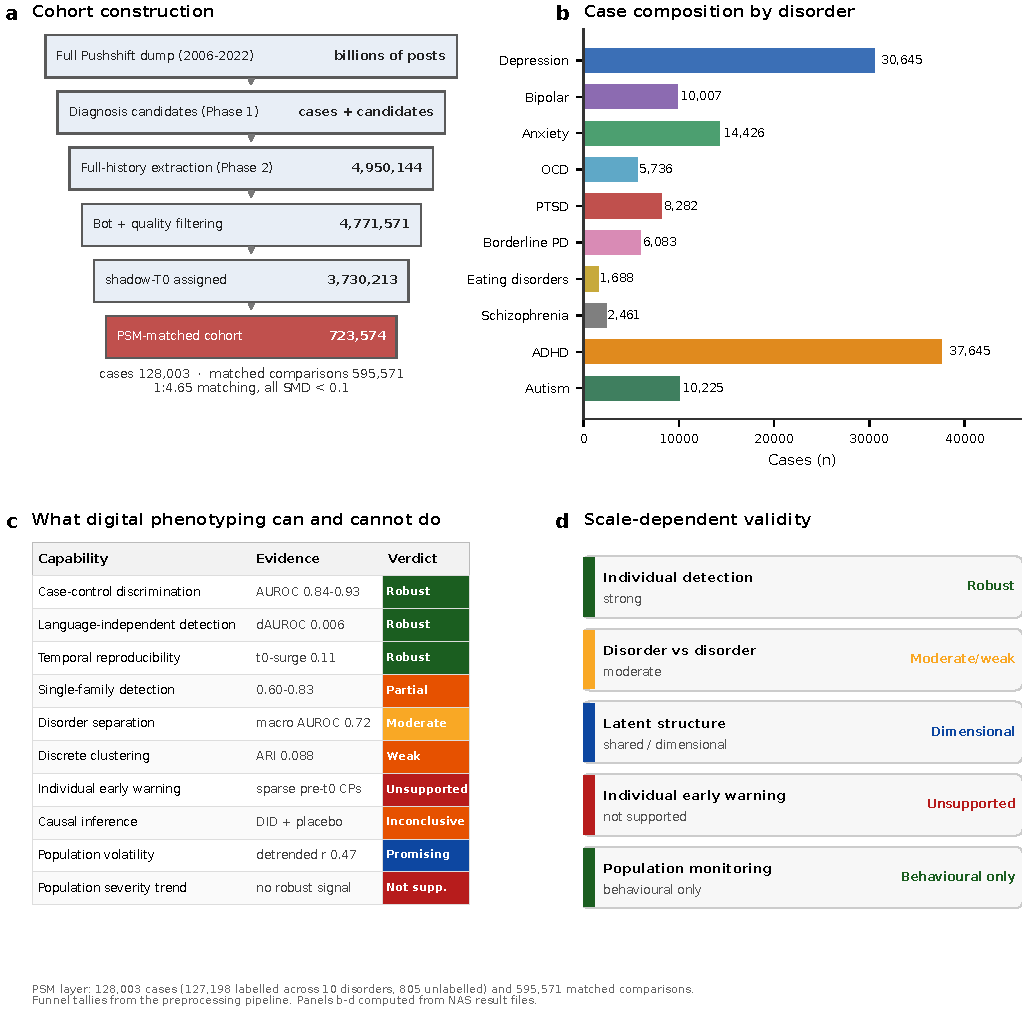
\includegraphics[width=\linewidth]{figures/fig1.pdf}
\caption{\textbf{Design of the study and the scale-dependent validity of digital phenotypes.}
\textbf{a}, Cohort-construction funnel from the full Reddit dump to the matched cohort.
\textbf{b}, Case composition by disorder in the matched layer. \textbf{c}, Capability map
summarising what digital phenotyping can and cannot do. \textbf{d}, Scale ladder from
individual detection to population monitoring with the verdict for each scale.}
\label{fig:design}
\end{figure}

\begin{figure}[htbp]\centering
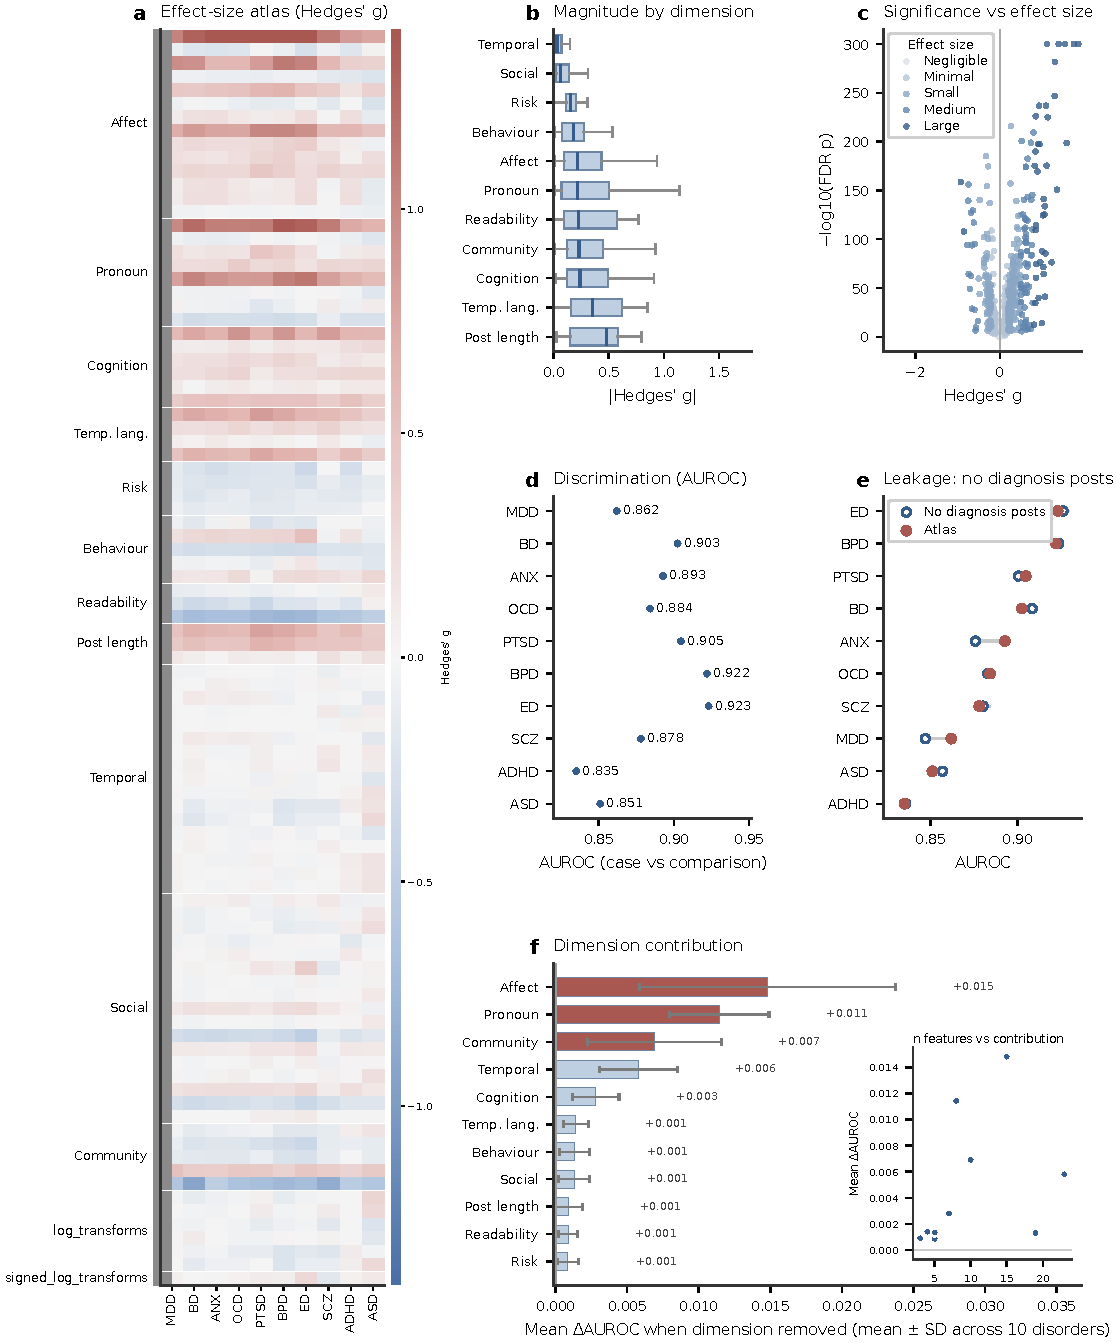
\includegraphics[width=\linewidth]{figures/fig2.pdf}
\caption{\textbf{A reproducible, multidimensional phenotype atlas.}
\textbf{a}, Feature--disorder effect-size atlas (Hedges' $g$). \textbf{b}, Effect magnitude by
feature dimension (box plots; whiskers, 1.5 $\times$ interquartile range; 860 effects, i.e. the
non-artefact feature--disorder tests restricted to the content feature dimensions; the atlas
itself comprises 930 non-artefact tests). \textbf{c}, Significance versus effect size (volcano plot of
$-\log_{10}$ false-discovery-rate $P$ against Hedges' $g$), points coloured by effect-size
category. \textbf{d}, Per-disorder case-versus-comparison AUROC (mean, s.d. across subsample
trials). \textbf{e}, Per-disorder AUROC of the full atlas (filled) versus after excluding
diagnosis-triggering posts (open; bar, range across trials). \textbf{f}, Dimension ablation
(mean $\Delta$AUROC when a dimension is removed, mean, s.d. across the ten disorders).}
\label{fig:atlas}
\end{figure}

\begin{figure}[htbp]\centering
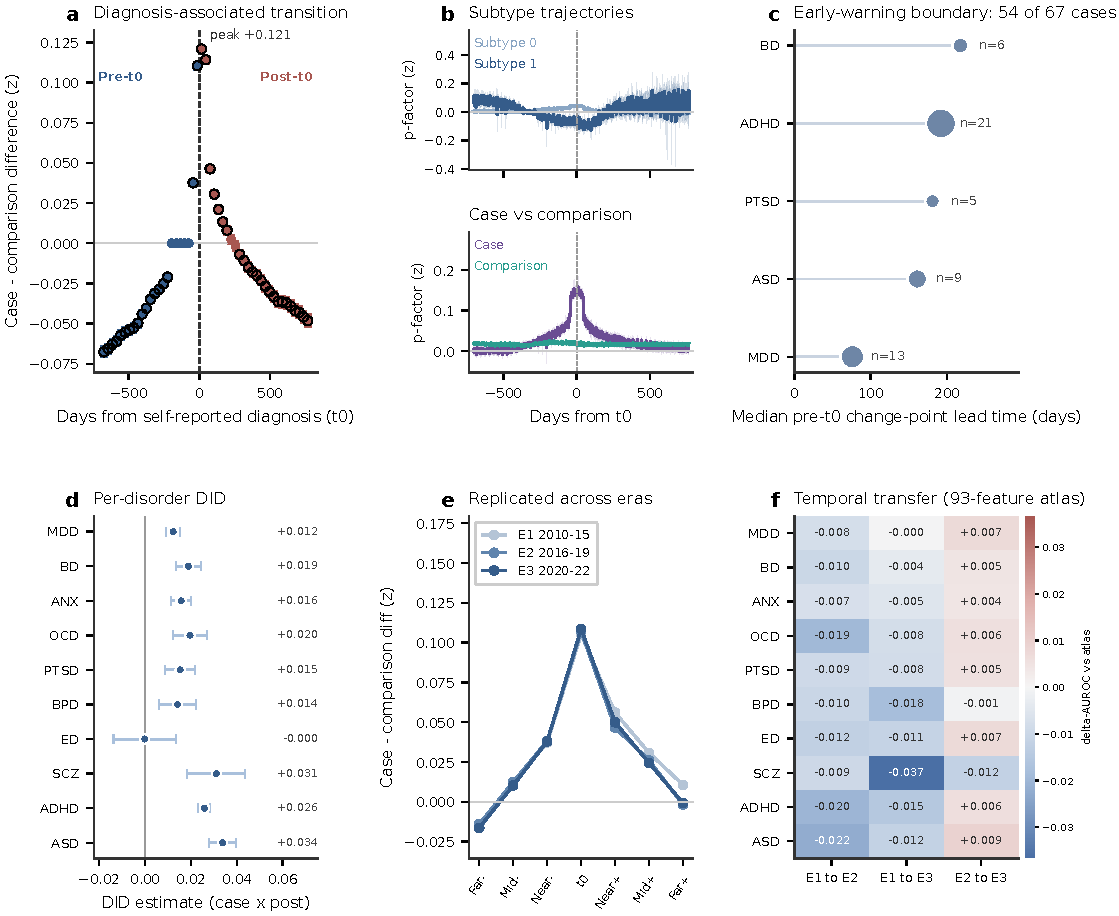
\includegraphics[width=\linewidth]{figures/fig3.pdf}
\caption{\textbf{A reproducible diagnosis-associated transition and the early-warning
boundary.} \textbf{a}, Event-study coefficients around the self-reported diagnosis date, with
95\% confidence intervals; these coefficients are descriptive and are not given a causal
interpretation. \textbf{b}, Two stacked sub-panels sharing the time axis: subtype
trajectories (top) and mean case-versus-comparison p-factor trajectories (bottom). \textbf{c},
Median pre-diagnosis change-point lead time by disorder (bubble area proportional to the number
of users with a pre-diagnosis change-point; 54 of the 67 cases shown; overall median lead
161 days). \textbf{d}, Per-disorder difference-in-differences estimates with confidence
intervals. \textbf{e}, Event-time profile replicated across three calendar eras. \textbf{f},
Classifier temporal transfer.}
\label{fig:temporal}
\end{figure}

\begin{figure}[htbp]\centering
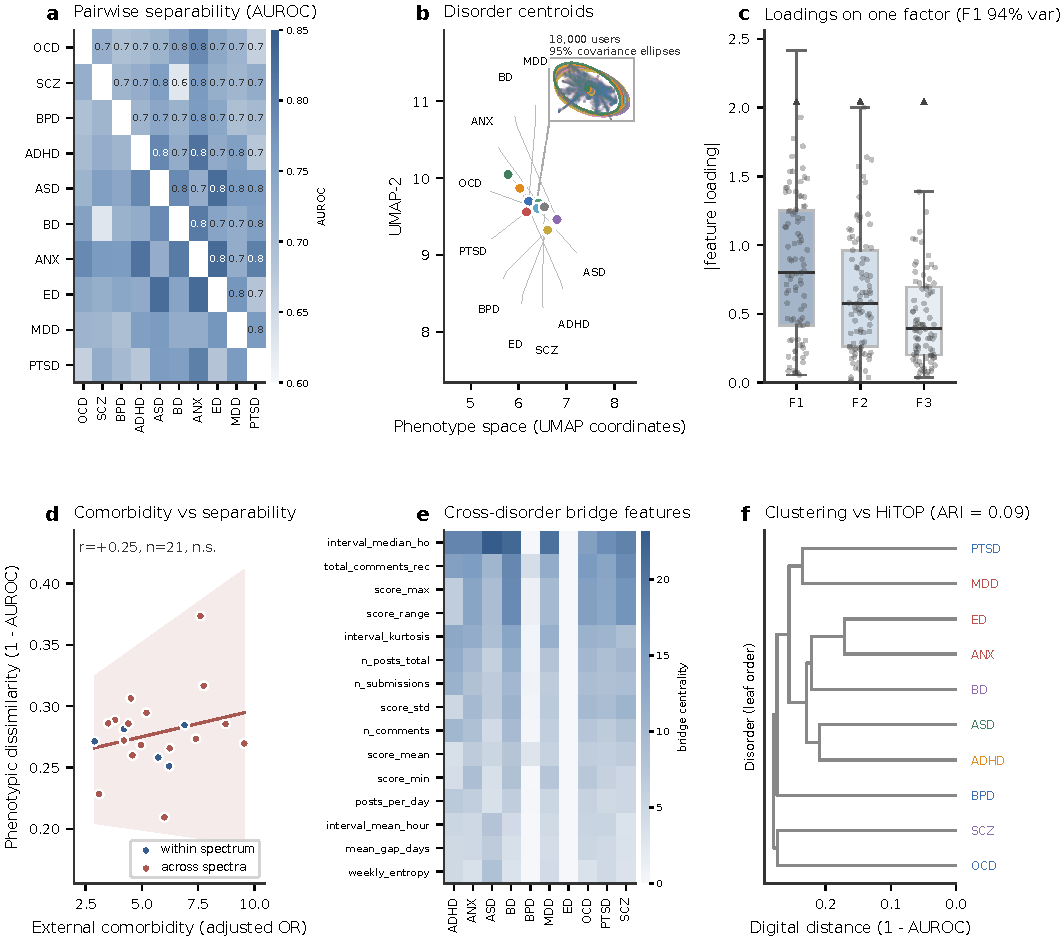
\includegraphics[width=\linewidth]{figures/fig4.pdf}
\caption{\textbf{Predominantly shared, dimensional cross-diagnostic structure.}
\textbf{a}, Pairwise case-versus-case AUROC heat map (rows and columns ordered by
average-linkage clustering on $1-$AUROC). \textbf{b}, Disorder centroids in phenotype space
with 95\% covariance ellipses; inset, the underlying 18{,}000-user embedding. \textbf{c},
Feature loadings on the three retained factors. \textbf{d}, Separability versus externally
sourced clinical comorbidity for the 21 published pairs (DOI-referenced odds-ratio subset);
the association was not statistically significant (Mantel $r=-0.247$, permutation $P=0.30$),
and is distinct from the positive same-cohort comorbidity association reported as internal
consistency only in \supfig{3}.
\textbf{e}, Cross-disorder bridge features. \textbf{f}, Hierarchical clustering versus HiTOP.}
\label{fig:structure}
\end{figure}

\begin{figure}[htbp]\centering
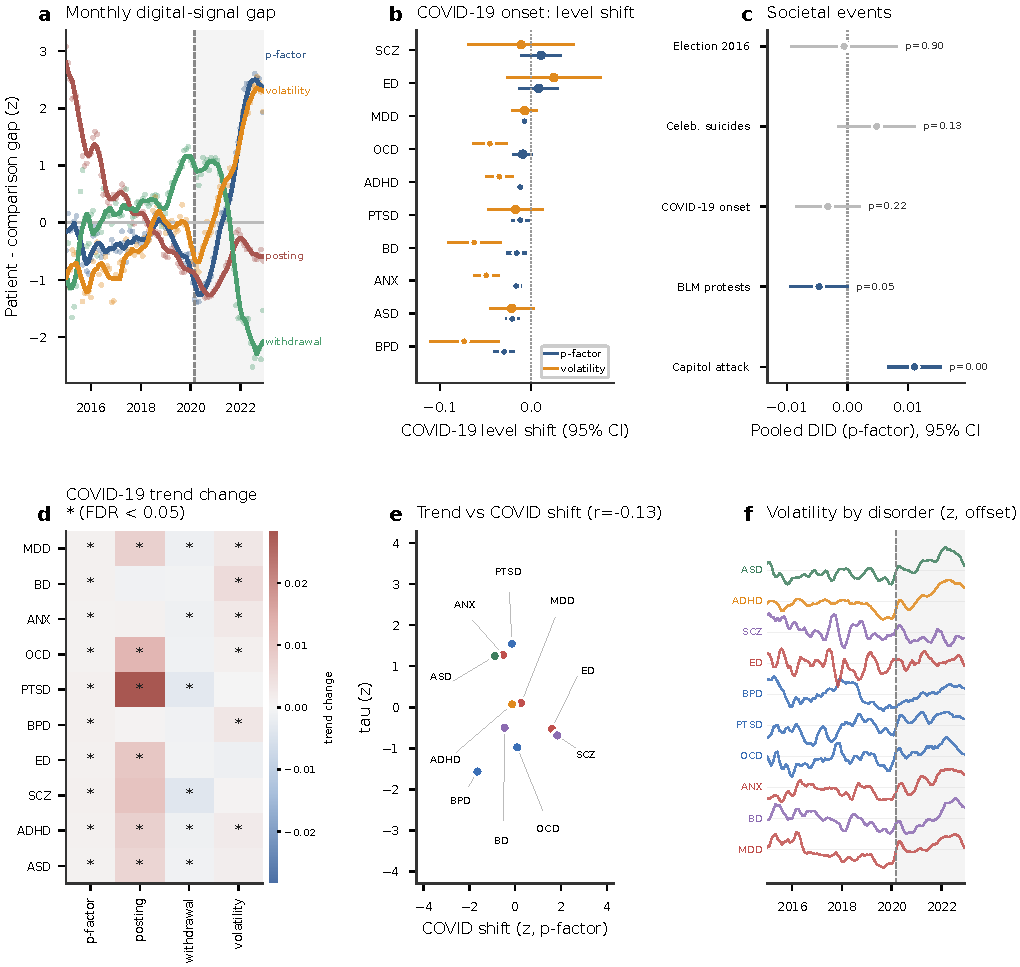
\includegraphics[width=\linewidth]{figures/fig5.pdf}
\caption{\textbf{Population-level behavioural signals around societal perturbations.}
\textbf{a}, Monthly case-minus-comparison gap for four digital signals (each standardised;
dots, monthly values; line, 6-month centred rolling mean), with the COVID-19 period shaded.
\textbf{b}, COVID-19 level shift per disorder for the p-factor and volatility signals (filled
markers, false-discovery-rate-adjusted $P<0.05$). \textbf{c}, Pooled difference-in-differences
estimates for five societal events. \textbf{d}, COVID-19 trend change by disorder and signal.
\textbf{e}, Long-term trend versus COVID-19 shift. \textbf{f}, Per-disorder volatility series.}
\label{fig:population}
\end{figure}

\begin{figure}[htbp]\centering
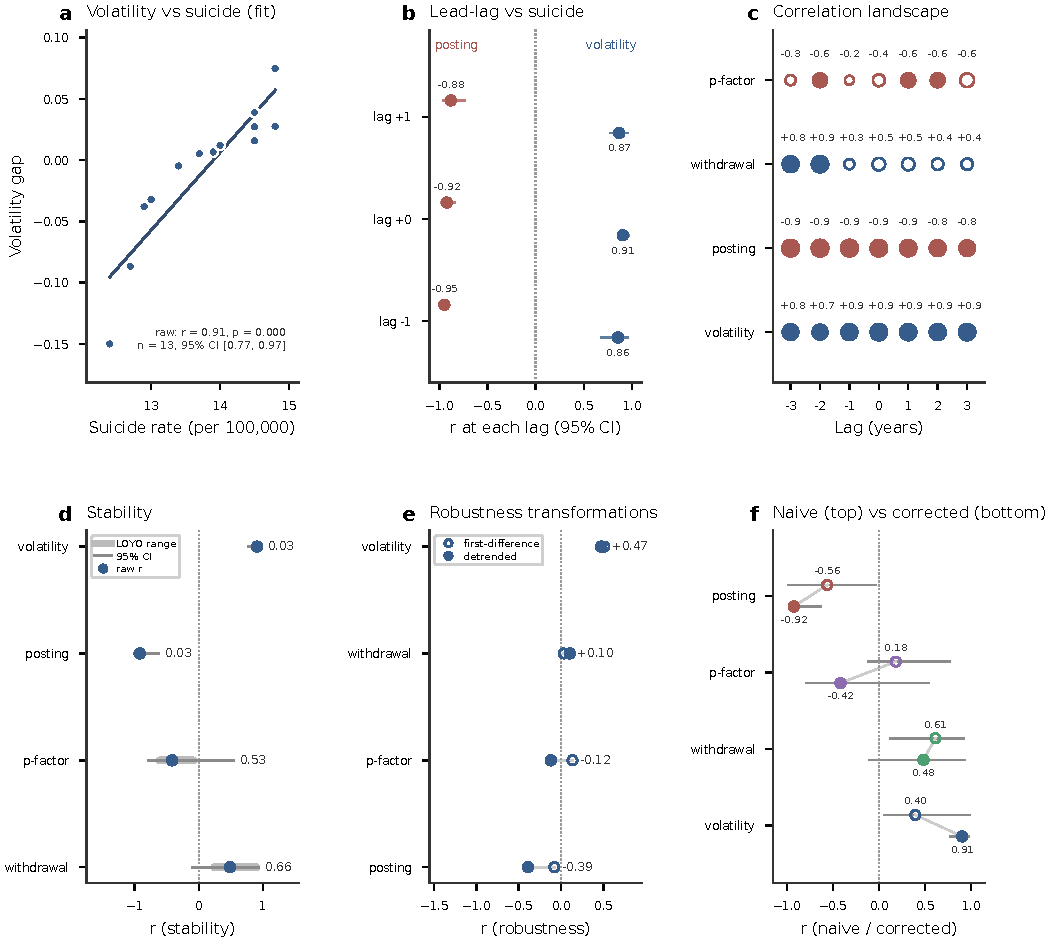
\includegraphics[width=\linewidth]{figures/fig6.pdf}
\caption{\textbf{External validation: behaviour versus language.}
\textbf{a}, Composition-corrected volatility gap against the national suicide rate (annual
series) with a least-squares fit; in-panel text gives the stored $r$, $P$, $n$ and bootstrap
95\% confidence interval. \textbf{b}, Lead--lag correlation at lags $-1/0/+1$ with confidence
intervals. \textbf{c}, Correlation landscape across signals and lags. \textbf{d},
Leave-one-year-out stability. \textbf{e}, First-difference versus detrended correlations.
\textbf{f}, Naive versus composition-corrected correlations.}
\label{fig:external}
\end{figure}

% ------------------------------------------------------------------ tables
\begin{table}[t]\centering\small
\caption{What digital phenotyping of mental disorders can and cannot do (capability map).}
\label{tab:capability}
\begin{tabular}{lll}
\toprule
Capability & Evidence & Verdict \\
\midrule
Case--control discrimination & AUROC 0.84--0.92 & Robust \\
Language-independent detection & mean $\Delta$AUROC 0.006 & Robust \\
Temporal reproducibility & $t_0$-surge 0.105--0.109 & Robust \\
Single-family detection & 0.60--0.83 & Partial \\
Disorder separation & mean pairwise AUROC 0.741 & Moderate \\
Discrete clustering & adjusted Rand index 0.088 & Weak \\
Individual early warning & 67 pre-$t_0$ change-points & Unsupported \\
Causal inference around diagnosis & difference-in-differences + placebo & Inconclusive \\
Population volatility monitoring & detrended $r$ 0.47 & Promising \\
Population severity/language trend & no robust signal & Not supported \\
\bottomrule
\end{tabular}
\end{table}

% ------------------------------------------------------------------ back matter
\section*{Back matter}
\paragraph*{Data availability.} Public Reddit posts were analysed in anonymised form. Cohort
summary statistics, the derived result tables underlying every figure, and the externally
sourced epidemiological series (CDC suicide mortality; SAMHSA NSDUH MDE) are available with the
manuscript; raw user-level data are not redistributed to protect privacy (Supplementary
Methods).
\paragraph*{Code availability.} The analysis pipeline (feature engineering, discrimination,
structure, trajectory, population and audit modules) and the figure-generation scripts are
available in the project repository.
\paragraph*{Ethics.} This study used publicly posted, anonymised data; the self-reported
diagnosis label is a behavioural proxy and not a clinical diagnosis, and no contact,
intervention or re-identification was performed. Ethical review exemption and data-governance
details are given in the Reporting Summary.
\paragraph*{Author contributions / Competing interests.} To be completed by the authors. The
authors declare no competing interests.

\begin{thebibliography}{99}\small
\bibitem{insel2017digital} Insel TR. Digital phenotyping. \emph{JAMA} \textbf{318}, 1215 (2017). \doi{10.1001/jama.2017.11295}
\bibitem{insel2018global} Insel TR. Digital phenotyping: a global tool for psychiatry. \emph{World Psychiatry} \textbf{17}, 276--277 (2018). \doi{10.1002/wps.20550}
\bibitem{onnela2016harnessing} Onnela JP, Rauch SL. Harnessing smartphone-based digital phenotyping. \emph{Neuropsychopharmacology} \textbf{41}, 1691--1696 (2016). \doi{10.1038/npp.2016.7}
\bibitem{torous2017dimensions} Torous J, Onnela JP, Keshavan M. New dimensions and new tools to realize the potential of RDoC. \emph{Transl. Psychiatry} \textbf{7}, e1053 (2017). \doi{10.1038/tp.2017.25}
\bibitem{braund2024hype} Braund TA. The continued hype and hope of digital phenotyping. \emph{Nat. Rev. Psychol.} \textbf{3}, 328--329 (2024). \doi{10.1038/s44159-024-00326-9}
\bibitem{giampetruzzi2026promise} Giampetruzzi E, Antonacci C, Gotlib IH. The promise of digital phenotyping for the early detection of risk for depression in adolescents. \emph{Nat. Ment. Health} \textbf{4}, 1193--1195 (2026). \doi{10.1038/s44220-026-00679-5}
\bibitem{adam2025smartphones} Adam D. Digital phenotyping using smartphones could help steer mental health treatment. \emph{PNAS} \textbf{122}, e2505700122 (2025). \doi{10.1073/pnas.2505700122}
\bibitem{lord2023autism} Lord C, Wilson RB. Digital phenotyping could help detect autism. \emph{Nat. Med.} \textbf{29}, 2408--2409 (2023). \doi{10.1038/s41591-023-02557-4}
\bibitem{dechoudhury2013predicting} De Choudhury M, Gamon M, Counts S, Horvitz E. Predicting depression via social media. \emph{ICWSM} \textbf{7}, 128--137 (2013). \doi{10.1609/icwsm.v7i1.14432}
\bibitem{coppersmith2014quantifying} Coppersmith G, Dredze M, Harman C. Quantifying mental health signals in Twitter. \emph{CLPsych} 51--60 (2014). \doi{10.3115/v1/w14-3207}
\bibitem{coppersmith2015adhd} Coppersmith G, Dredze M, Harman C, Hollingshead K. From ADHD to SAD. \emph{CLPsych} 1--10 (2015). \doi{10.3115/v1/w15-1201}
\bibitem{eichstaedt2018facebook} Eichstaedt JC \emph{et al.} Facebook language predicts depression in medical records. \emph{PNAS} \textbf{115}, 11203--11208 (2018). \doi{10.1073/pnas.1802331115}
\bibitem{guntuku2017detecting} Guntuku SC \emph{et al.} Detecting depression and mental illness on social media. \emph{Curr. Opin. Behav. Sci.} \textbf{18}, 43--49 (2017). \doi{10.1016/j.cobeha.2017.07.005}
\bibitem{orben2019association} Orben A, Przybylski AK. The association between adolescent well-being and digital technology use. \emph{Nat. Hum. Behav.} \textbf{3}, 173--182 (2019). \doi{10.1038/s41562-018-0506-1}
\bibitem{panayiotou2023time} Panayiotou M \emph{et al.} Time spent on social media among the least influential factors in adolescent mental health. \emph{Nat. Ment. Health} \textbf{1}, (2023). \doi{10.1038/s44220-023-00063-7}
\bibitem{pennebaker1999linguistic} Pennebaker JW, King LA. Linguistic styles: language use as an individual difference. \emph{J. Pers. Soc. Psychol.} \textbf{77}, 1296--1312 (1999). \doi{10.1037/0022-3514.77.6.1296}
\bibitem{pennebaker2003psychological} Pennebaker JW, Mehl MR, Niederhoffer KG. Psychological aspects of natural language use. \emph{Annu. Rev. Psychol.} \textbf{54}, 547--577 (2003). \doi{10.1146/annurev.psych.54.101601.145041}
\bibitem{rude2004language} Rude S, Gortner EM, Pennebaker JW. Language use of depressed and depression-vulnerable college students. \emph{Cogn. Emot.} \textbf{18}, 1121--1133 (2004). \doi{10.1080/02699930441000030}
\bibitem{stirman2001word} Stirman SW, Pennebaker JW. Word use in the poetry of suicidal and nonsuicidal poets. \emph{Psychosom. Med.} \textbf{63}, 517--522 (2001). \doi{10.1097/00006842-200107000-00001}
\bibitem{almosaiwi2018absolute} Al-Mosaiwi M, Johnstone T. Elevated use of absolutist words is a marker specific to anxiety, depression and suicidal ideation. \emph{Clin. Psychol. Sci.} \textbf{6}, 529--542 (2018). \doi{10.1177/2167702617747074}
\bibitem{dechoudhury2016discovering} De Choudhury M \emph{et al.} Discovering shifts to suicidal ideation from mental health content in social media. \emph{CHI} 2098--2110 (2016). \doi{10.1145/2858036.2858207}
\bibitem{schwartz2013personality} Schwartz HA \emph{et al.} Personality, gender and age in the language of social media. \emph{PLoS ONE} \textbf{8}, e73791 (2013). \doi{10.1371/journal.pone.0073791}
\bibitem{kern2014online} Kern ML \emph{et al.} The online social self: an open vocabulary approach to personality. \emph{Assessment} \textbf{21}, 158--169 (2014). \doi{10.1177/1073191113514104}
\bibitem{eichstaedt2015heart} Eichstaedt JC \emph{et al.} Psychological language on Twitter predicts county-level heart disease mortality. \emph{Psychol. Sci.} \textbf{26}, 159--169 (2015). \doi{10.1177/0956797614557867}
\bibitem{brown2018replicationstatements} Brown NJL, Coyne JC. Replication statements in psychology. \emph{Preprint} (2018). \doi{10.31234/osf.io/dursw}
\bibitem{rai2024race} Rai S \emph{et al.} Key language markers of depression on social media depend on race. \emph{PNAS} \textbf{121}, e2319837121 (2024). \doi{10.1073/pnas.2319837121}
\bibitem{defreitas2024black} De Freitas J \emph{et al.} Do ``Black individuals'' really display no linguistic markers of depression? \emph{PNAS} \textbf{121}, e2410997121 (2024). \doi{10.1073/pnas.2410997121}
\bibitem{wang2024llm} Wang Y. Large language models for depression prediction. \emph{PNAS} \textbf{121}, e2409757121 (2024). \doi{10.1073/pnas.2409757121}
\bibitem{hur2024sentiment} Hur JK \emph{et al.} Language sentiment predicts changes in depressive symptoms. \emph{PNAS} \textbf{121}, e2321321121 (2024). \doi{10.1073/pnas.2321321121}
\bibitem{caspi2014p} Caspi A \emph{et al.} The p factor: one general psychopathology factor. \emph{Clin. Psychol. Sci.} \textbf{2}, 119--137 (2014). \doi{10.1177/2167702613497473}
\bibitem{kotov2017hitop} Kotov R \emph{et al.} The Hierarchical Taxonomy of Psychopathology (HiTOP). \emph{J. Abnorm. Psychol.} \textbf{126}, 454--477 (2017). \doi{10.1037/abn0000258}
\bibitem{rodriguezseijas2023diversity} Rodriguez-Seijas C \emph{et al.} Diversity and HiTOP. \emph{Nat. Rev. Psychol.} \textbf{2}, (2023). \doi{10.1038/s44159-023-00200-0}
\bibitem{pnas2023pfactor} ``P factor'' could open an important window on core attributes of mental health maladies. \emph{PNAS} \textbf{120}, e2316297120 (2023). \doi{10.1073/pnas.2316297120}
\bibitem{braghieri2022social} Braghieri L, Levy R, Makarin A. Social media and mental health. \emph{Am. Econ. Rev.} \textbf{112}, 3660--3693 (2022). \doi{10.1257/aer.20211218}
\bibitem{allcott2020welfare} Allcott H \emph{et al.} The welfare effects of social media. \emph{Am. Econ. Rev.} \textbf{110}, 629--676 (2020). \doi{10.1257/aer.20190658}
\bibitem{shi2026protests} Shi J \emph{et al.} Interpersonal conflicts, social media use and depression associated with protests. \emph{Nat. Med.} \textbf{32}, (2026). \doi{10.1038/s41591-025-04145-0}
\bibitem{roozenbeek2026protests} Roozenbeek J, Ma I. Political protests, social media use and mental well-being. \emph{Nat. Med.} \textbf{32}, (2026). \doi{10.1038/s41591-025-04110-x}
\bibitem{skeggs2025interventions} Skeggs A, Orben A. Social media interventions to improve well-being. \emph{Nat. Hum. Behav.} \textbf{9}, (2025). \doi{10.1038/s41562-025-02167-9}
\bibitem{pearson2025smartphones} Pearson H. Do smartphones and social media really harm teens' mental health? \emph{Nature} \textbf{640}, 30--33 (2025). \doi{10.1038/d41586-025-00933-3}
\bibitem{capraro2025llmwellbeing} Simulating human well-being with large language models. \emph{PNAS} \textbf{122}, e2519394122 (2025). \doi{10.1073/pnas.2519394122}
\bibitem{hitopnetwork2023} A transdiagnostic network for psychiatric illness derived from atrophy and lesions. \emph{Nat. Hum. Behav.} \textbf{7}, 166--174 (2023). \doi{10.1038/s41562-022-01501-9}
\bibitem{fradkin2025language} Fradkin I \emph{et al.} Latent mechanisms of language disorganization relate to specific dimensions of psychopathology. \emph{Nat. Ment. Health} \textbf{3}, (2025). \doi{10.1038/s44220-024-00351-w}
\bibitem{fassi2025adolescents} Fassi L \emph{et al.} Social media use in adolescents with and without mental health conditions. \emph{Nat. Hum. Behav.} \textbf{9}, (2025). \doi{10.1038/s41562-025-02134-4}
\bibitem{hutto2014vader} Hutto CJ, Gilbert E. VADER: a parsimonious rule-based model for sentiment analysis of social media text. \emph{ICWSM} \textbf{8}, 216--225 (2014). \doi{10.1609/icwsm.v8i1.14550}
\bibitem{benjamini1995controlling} Benjamini Y, Hochberg Y. Controlling the false discovery rate. \emph{J. R. Stat. Soc. B} \textbf{57}, 289--300 (1995). \doi{10.1111/j.2517-6161.1995.tb02031.x}
\bibitem{rosenbaum1983central} Rosenbaum PR, Rubin DB. The central role of the propensity score in observational studies. \emph{Biometrika} \textbf{70}, 41--55 (1983). \doi{10.1093/biomet/70.1.41}
\bibitem{stuart2010matching} Stuart EA. Matching methods for causal inference: a review. \emph{Stat. Methods Med. Res.} \textbf{19}, 71--101 (2010). \doi{10.1177/0962280209105024}
\bibitem{tibshirani1996regression} Tibshirani R. Regression shrinkage and selection via the lasso. \emph{J. R. Stat. Soc. B} \textbf{58}, 267--288 (1996). \doi{10.1111/j.2517-6161.1996.tb02080.x}
\bibitem{killick2012optimal} Killick R, Fearnhead P, Eckley IA. Optimal detection of changepoints with a linear computational cost. \emph{JASA} \textbf{107}, 1590--1598 (2012). \doi{10.1080/01621459.2012.737745}
\bibitem{truong2020selective} Truong C, Oudre L, Vayatis N. Selective review of offline change point detection methods. \emph{Signal Processing} \textbf{167}, 107299 (2020). \doi{10.1016/j.sigpro.2019.107398}
\bibitem{dempster1977maximum} Dempster AP, Laird NM, Rubin DB. Maximum likelihood from incomplete data via the EM algorithm. \emph{J. R. Stat. Soc. B} \textbf{39}, 1--22 (1977). \doi{10.1111/j.2517-6161.1977.tb01600.x}
\bibitem{friedman2008sparse} Friedman J, Hastie T, Tibshirani R. Sparse inverse covariance estimation with the graphical lasso. \emph{Biostatistics} \textbf{9}, 432--441 (2008). \doi{10.1093/biostatistics/kxm045}
\bibitem{cameron2011robust} Cameron AC, Gelbach JB, Miller DL. Robust inference with multiway clustering. \emph{J. Bus. Econ. Stat.} \textbf{29}, 238--249 (2011). \doi{10.1198/jbes.2010.07136}
\bibitem{mcinnes2018umap} McInnes L, Healy J, Melville J. UMAP: uniform manifold approximation and projection. \emph{arXiv:1802.03426} (2018).
\bibitem{pedregosa2011scikit} Pedregosa F \emph{et al.} Scikit-learn: machine learning in Python. \emph{J. Mach. Learn. Res.} \textbf{12}, 2825--2830 (2011).
\bibitem{apa2013dsm5} American Psychiatric Association. \emph{Diagnostic and Statistical Manual of Mental Disorders} 5th edn (American Psychiatric Association, 2013).
\bibitem{pennebaker2015liwc} Pennebaker JW, Boyd RL, Jordan K, Blackburn K. \emph{The Development and Psychometric Properties of LIWC2015} (University of Texas at Austin, 2015).
\bibitem{mohammad2013nrc} Mohammad SM, Turney PD. Crowdsourcing a word--emotion association lexicon. \emph{Comput. Intell.} \textbf{29}, 436--465 (2013). \doi{10.1111/j.1467-8640.2012.00460.x}
\end{thebibliography}

\end{document}
